\chapter{Evaluating the Proof-of-Concept SOSAA RSM} \label{txt:icarus-evaluation-chapter}

This thesis project started with the motivation of constructing a response surface model (RSM) for the SOSAA model (see \Cref{txt:sosaa-model}). In particular, the initial goal was to efficiently support big data analysis on SOSAA using an RSM. However, we wanted to go even further and train an RSM as fast as possible with as little data as possible to account for the dynamic research environment in which SOSAA is being developed and enable the RSM to be used to perform preliminary analysis on fresh SOSAA runs.

A single SOSAA trajectory run only takes around three hours using ten CPU cores. Since an RSM can only provide approximations, the value of an RSM that takes around an hour to train and predict would likely be of little value. Suppose that the training and prediction time was instead cut down to just a few minutes. This speedup could radically change the SOSAA model workflow. In particular, such a fast SOSAA RSM could be integrated into an interactive research workflow that would add value to the SOSAA model by allowing researchers to explore the feature space around existing runs to carefully design the inputs for the next SOSAA model runs. Pre-training a highly accurate deep neural network on a vast database of diverse model runs is enticing. However, the vastness of SOSAA's input parameter space means that researchers could still easily hit the boundary of the model's ID training data manifold with new trajectories. Combined with the continuous changes to SOSAA, such a neural network would require frequent and costly retraining. Therefore, this project's initial goal was to only use a single trajectory to train a local RSM.

However, as \Cref{txt:icarus-chapter} has outlined, training a traditional RSM with little data is dangerous since it may produce a model that does not generalise beyond its training data set but also gives little indication for when it fails. This problem motivated us to research \textit{prudent} response surface models and design the Icarus RSM architecture (see \Cref{txt:icarus-rsm}), which produces confidence scores and uncertainty levels alongside each prediction. These confidences and uncertainties can then be propagated through any analysis to the final results (see \Cref{txt:icarus-propagation}). Our literature review in \Cref{txt:background-chapter} and experiments in \Cref{txt:ood-detection-chapter}, \Cref{txt:prediction-chapter}, and \Cref{txt:uncertainty-chapter} have explored the three components of Icarus, an out-of-distribution (OOD) detector, a prediction model, and an uncertainty quantifier, in detail. These experiments form the primary contribution of this thesis.

\newpar In this chapter, we come full circle to the initial motivation of this project and attempt to implement a SOSAA RSM using our insights from the prior experiments. However, it is worth noting that this SOSAA RSM is only a proof-of-concept that should serve as a baseline implementation for future research. Furthermore, we expect that better implementations for each component can be identified, particularly for the prediction model, and especially if the training time and runtime constraints for the SOSAA RSM that have guided this project are changed. Keeping these motivations and limitations in mind, we have chosen the following components for the SOSAA RSM proof-of-concept implementation, which are also shown in \Cref{fig:sosaa-rsm}:

For out-of-distribution (OOD) detection and confidence scoring, we approximate an auto-associative network using truncated principal component analysis (PCA), where only the first $k$ principal components that explain $95\%$ of the training data variance are kept (see \Cref{txt:truncated-pca} and \Cref{txt:ood-logistic-scoring}). The per-feature reconstruction errors from compressing and decompressing the inputs using PCA are transformed into a scalar score using the Mahalanobis distance. We use the fast gradient sign method on the reconstruction errors to synthesise OOD inputs (see \Cref{txt:adversarial-ood-synthesis-analysis}). Finally, the Mahalanobis distances of the ID training inputs and the synthetic OOD samples are used to train a logistic regression model, which outputs the final confidence score (see \Cref{txt:ood-logistic-scoring}).

We evaluate both random forests (RFs, see \Cref{txt:ensembles-decision-tree-random-forest}) and Pairwise Difference Regression with Random Forests (PADRE-RF, see \Cref{txt:padre-rf}) as prediction models for the SOSAA RSM. Both are ensemble methods that combine the predictions from several (here sixteen) decision trees. As in \Cref{txt:model-evaluation}, we only allow the random forests to look at one-third of the features at each split during training and require at least five training samples per leaf node to discourage overfitting \cite{statistical-learning-2009}. At test time, the predictions from each tree in the random forest are averaged. For PADRE-RF, each difference prediction is made relative to a randomly chosen training data anchor example. We repeat this random prediction four times and use uncertainty and confidence propagation as described in \Cref{txt:icarus-propagation} to combine them into one less noisy PADRE-RF prediction.

We also use the ensemble predictions of the prediction model to quantify the prediction uncertainty (see \Cref{txt:uncertainty-ensemble-methods}). In detail, the uncertainty level $\sigma$ is estimated as the standard deviation across all predictions in the ensemble. For random forests, these uncalibrated uncertainties are output directly. For PADRE-RF, we apply the CRUDE \cite{not-crude-uncertainty-2020} calibration to the uncertainty levels, which provided better results in \Cref{fig:uncertainty-padre-residual}.

\begin{figure}[H]
    \centering
    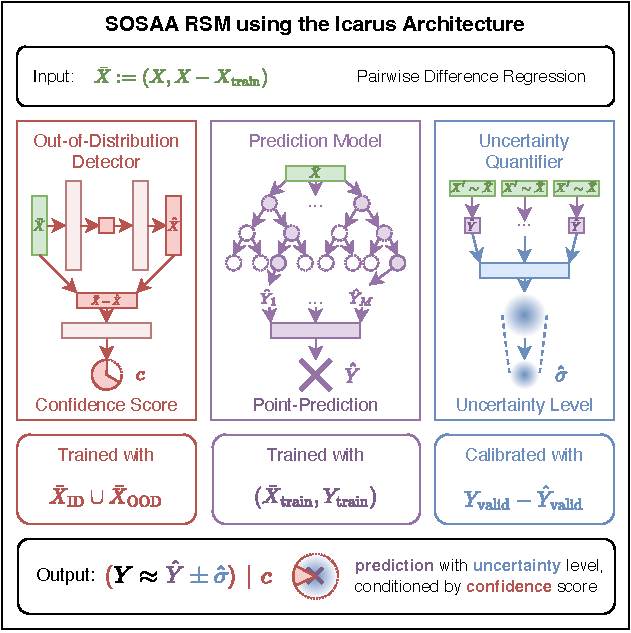
\includegraphics[width=0.95\textwidth]{evaluation/figures/sosaa-rsm.pdf}
    \caption[Overview of the prudent SOSAA RSM Architecture]{Overview of the prudent SOSAA RSM built with the Icarus Architecture, which consists of three components: the out-of-distribution detector based auto-associative truncated PCA using logistic regression for confidence scoring (see \Cref{txt:ood-logistic-scoring}), the prediction model using Pairwise Difference Regression with Random Forests (see \Cref{txt:padre-rf}), and the Uncertainty Quantifier that repeatedly samples the prediction model (see \Cref{txt:uncertainty-ensemble-methods}) and calibrates the ensemble uncertainty using the CRUDE method \cite{not-crude-uncertainty-2020}. The SOSAA RSM produces predictions with normal-distributed uncertainty, which are conditioned on the confidence score. In this diagram, a confidence circle that fully blocks the prediction and uncertainty represents zero confidence that the input is in-distribution.}
    \label{fig:sosaa-rsm}
\end{figure}

\noindent We use the \textbf{M}ean \textbf{A}bsolute \textbf{E}rror and $R^2$ score, all calculated in $\log_{10}(CCN)$ space, for the following evaluations. Since the MAE is in log-space, it can also be interpreted as a mean relative error in linear space. Note that while lower errors are better, the $R^2$ score of a model is $1.0$ at best but can be arbitrarily negative. The SOSAA RSM implements the Icarus RSM architecture and thus reports predictions with confidence scores and uncertainty levels. Thus, we can use confidence and uncertainty propagation (see \Cref{txt:icarus-propagation}) to obtain the MAE's and $R^2$'s confidence and uncertainty. It is important to remember that any result and its uncertainty are conditioned on the confidence value and already integrate the confidence and uncertainty of all predictions.

In the following sections, the performance of the proof-of-concept SOSAA RSM implementation is evaluated from several perspectives, always comparing random forests against PADRE-RF. First, \Cref{txt:clump-generalisation} uses clumped train-test splits to examine how much each RSM relies on spatiotemporal memory of the training data. Second, \Cref{txt:temporal-generalisation} showcases how the RSM performs on temporally adjacent trajectories that should thus have similar inputs. Third, \Cref{txt:trajectory-generalisation} explores how an RSM trained on one trajectory generalises across five other trajectories that showcase different scenarios and thus cover a more extensive range of the input space. Finally, \Cref{txt:perturbation-generalisation} pushes the RSM to its limit and tests how well a model trained on a single trajectory can predict a local perturbation to this trajectory. In all these evaluations, six different trajectories are used to compare each model's performance across different scenarios. Please refer back to \Cref{txt:six-trajectories} for a description of these six trajectories. Finally, \Cref{txt:sosaa-rsm-conclusions} summarises the insights we have gained from these evaluations.

\section{Performance on Clumped Train-Test Splits} \label{txt:clump-generalisation}

First, we examine how the SOSAA RSM performs on the disjoint test data from its training trajectory. In particular, we test how much the prediction models have learned in contrast to relying on just spatiotemporal memory. Suppose the train-test split of the training trajectory is created using independently and identically distributed (iid) randomness. In that case, every test point is likely surrounded by many training data points between which the model can simply interpolate. \Cref{txt:clumped-train-test-split} has introduced our clumping method, which instead (1) puts all samples from the same time step into either the training or test dataset and (2) puts adjacent timesteps both into the same set as clumping increases. While a clumping factor of $0\%$ is equivalent to iid sampling on the time steps, $100\%$ clumping puts \textit{all} samples into the same set.

\begin{figure}[H]
    \centering
    \begin{subfigure}
        \centering
        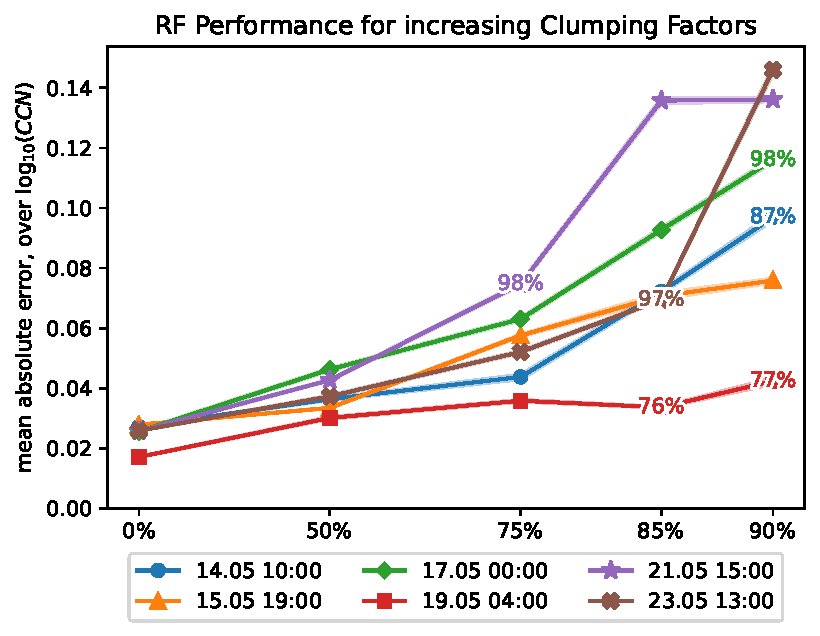
\includegraphics[width=0.425\textwidth]{evaluation/figures/results/clumped-generalisation-rf.pdf}
    \end{subfigure}
    \begin{subfigure}
        \centering
        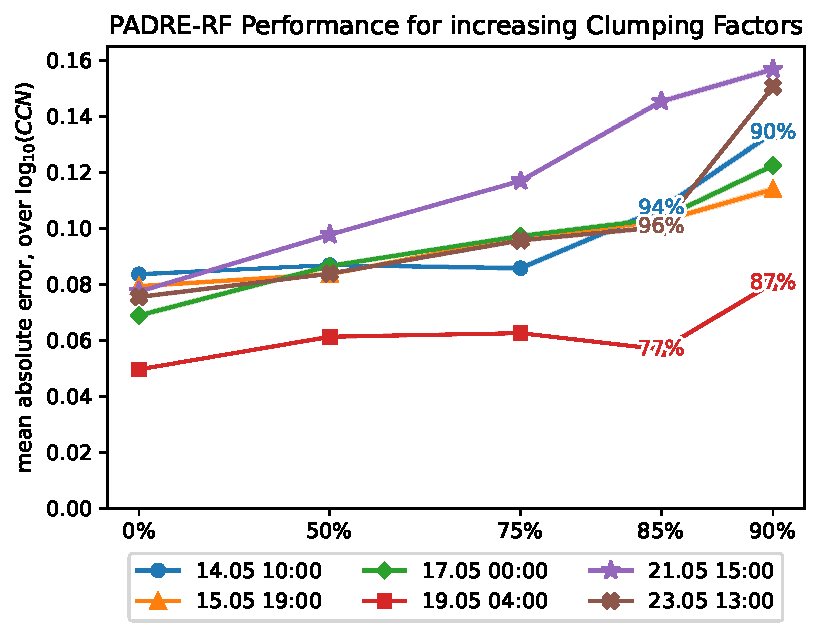
\includegraphics[width=0.425\textwidth]{evaluation/figures/results/clumped-generalisation-padre-rf.pdf}
    \end{subfigure}

    \caption[Evaluation of the SOSAA RSM for increasing Clumping Factors]{Evaluation of the SOSAA RSM for increasing clumping factors, with SOSAA-RF on the left and SOSAA-PADRE-RF on the right. The mean absolute error on the test set is plotted on the y-axis against the clumping percentage on the x-axis. Note that the x-axis is not linear but logarithmic. The propagated uncertainty level $\mu_{\text{MAE}} \pm \sigma_{\text{MAE}}$ is shown as a filled area around the similarly coloured MAE lines, which is only visible if the uncertainty is non-negligible. The confidence of each MAE estimate is also given if it is below $99\%$.}
    \label{fig:sosaa-rsm-clumping}
\end{figure}

\noindent \Cref{fig:sosaa-rsm-clumping} compares the performance of the RF-based SOSAA RSM to the one built with PADRE-RF. We can observe that increasing clumping significantly increases the random forest's prediction error, indicating that it may rely on some spatiotemporal memory. In contrast, the SOSAA-PADRE-RF performs with initially significantly higher but much more slowly growing error even as clumping increases, which hints that this RSM might be more robust. It is also worth noting that uncertainty is very low across all MAE estimates and that confidence is mostly high. While confidence is more likely to dip below $99\%$ on higher clumping factors, no direct correlation between prediction error and confidence is visible.

We use $75\%$ clumping in all following analyses to discourage relying excessively on spatiotemporal memory.

\section{Performance on Time-Adjacent Trajectories} \label{txt:temporal-generalisation}

In this second evaluation, we expand our view beyond the training trajectory. We examine how each of the RMs performs on the trajectories that arrived right before or after their training trajectory. Under stable conditions, the trajectory path does not change significantly across several hours, and the RSM should thus be able to generalise well temporally. We know from \Cref{fig:six-trajectories-maps} that conditions were stable for most trajectories with a few notable exceptions. For example, the $t-4\text{h}$ trajectory for 15.05.2018 19:00 UTC, all later trajectories after 19.05.2018 04:00 UTC, and all adjacent trajectories for 23.05.2018 13:00 UTC show significant deviations from the training trajectory path. Thus, seeing higher prediction errors in these cases would not be unexpected.

\begin{figure}[H]
    \centering
    \begin{subfigure}
        \centering
        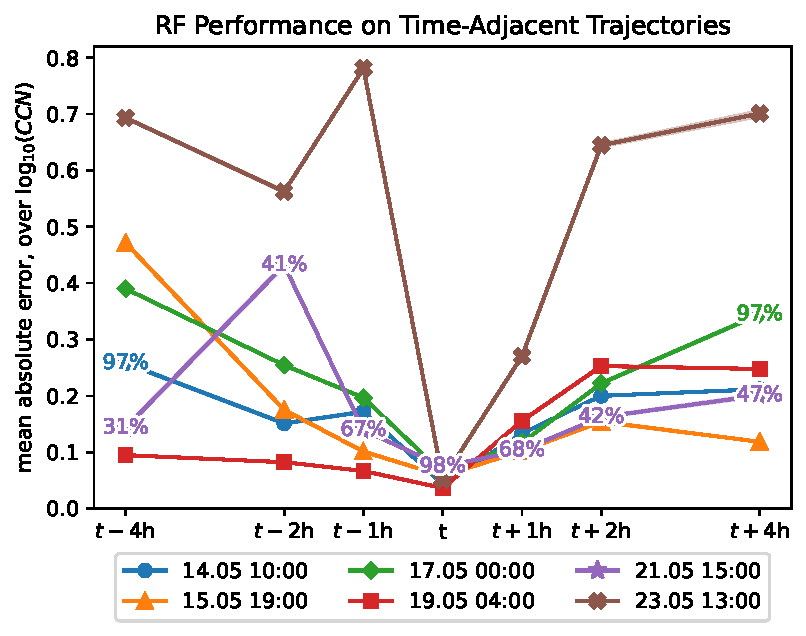
\includegraphics[width=0.425\textwidth]{evaluation/figures/results/temporal-generalisation-rf.pdf}
    \end{subfigure}
    \begin{subfigure}
        \centering
        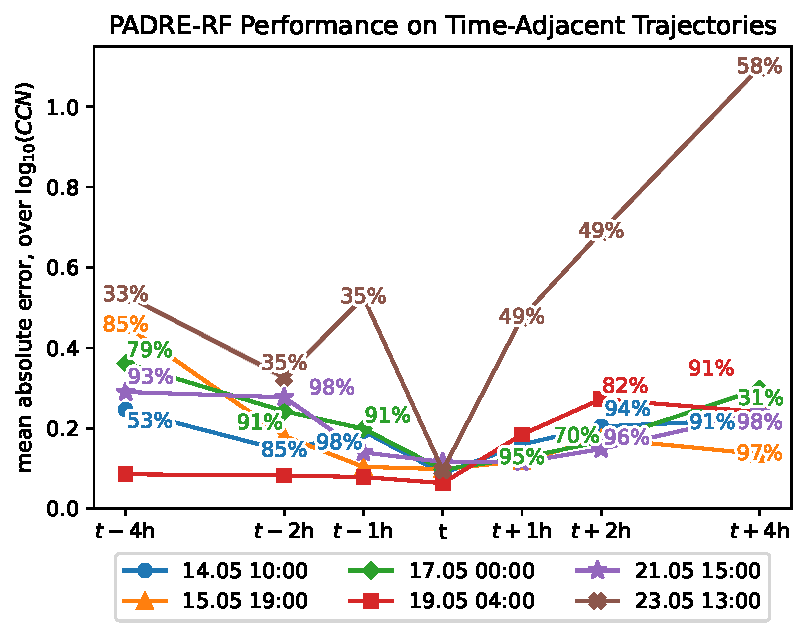
\includegraphics[width=0.425\textwidth]{evaluation/figures/results/temporal-generalisation-padre-rf.pdf}
    \end{subfigure}

    \caption[Evaluation of the SOSAA RSM on Time-Adjacent Trajectories]{Evaluation of the SOSAA RSM on time-adjacent trajectories, with SOSAA-RF on the left and SOSAA-PADRE-RF on the right. The mean absolute error on the test set is plotted on the y-axis against the trajectory arrival time offset on the x-axis. The propagated uncertainty level $\mu_{\text{MAE}} \pm \sigma_{\text{MAE}}$ is shown as a filled area around the similarly coloured MAE lines. The confidence of each MAE estimate is also given if it is below $99\%$. Overlap between the confidence labels is avoided using the \texttt{adjustText} Python package by \textcite{matplotlib-adjust-text-2023}.}
    \label{fig:sosaa-rsm-temporal}
\end{figure}

\noindent \Cref{fig:sosaa-rsm-temporal} compares the temporal generalisation abilities of the RF- and PADRE-RF-based SOSAA RSM implementations. As foreseen above, trajectories with significant changes to their paths over time have higher prediction errors. For instance, the trajectory on 23.05.2018 shifts geographically from a path that travels to Great Britain to one that either stays over Norway and Sweden or one that crosses the Atlantic near Greenland (see \Cref{fig:six-trajectories-maps}), and both RF and PADRE-RF struggle the most with this test case. Outside this case, both prediction models perform similarly well with PADRE-RF, sometimes even producing lower prediction errors. For the 23.05. trajectory, PADRE-RF is especially confused by the scenario shift in later-arriving trajectories that travel across the Atlantic. However, it predicts the shift to the Nordics in earlier trajectories better, whereas SOSAA-RF performs equally badly in both cases. While uncertainties are again low, we can now observe the out-of-distribution detector in action. Specifically, it fails on the 23.05.2018 trajectory for the random forest but does identify it as suspicious for PADRE-RF. Why is there a difference even though both SOSAA RSM implementations use the same OOD detector? It is worth remembering that while random forests predict directly on the input $X$, our PADRE-RF implementation takes $(X, X-X_{\text{train}})$ as input instead. The OOD detectors naturally use the same input as the prediction models. Therefore, this experiment suggests that explicitly taking differences to the training data into account can help with OOD detection.

\section{Generalisation to Other Trajectories} \label{txt:trajectory-generalisation}

After analysing the performance of the SOSAA RSM on time-adjacent trajectories, this section again broadens the scope. Each of the six RSMs, trained on one of the six trajectories (see \Cref{txt:six-trajectories}), is now evaluated on the other five trajectories. Since the scenarios represented across the six trajectories differ and the RMs have already struggled with some of the time-adjacent trajectories, we expect some RSMs to fail at generalising to the others. Therefore, we are especially interested in how the OOD detector performs.

\Cref{fig:sosaa-rsm-trajectories} compares the mean absolute errors (first row) and $R^2$ scores (second row) of the RF (left) and PADRE-RF-based (right) RSMs. The RF-RSMs all perform very well on their training trajectory but have increased errors elsewhere. The OOD detector successfully predicts lower confidence for the higher error and lower $R^2$ score trajectories. The 19.05. and 21.05. trajectories seem to be particularly out-of-distribution for all other runs, most likely since they spend more time over the Atlantic than the others. In contrast, the RSM trained on the 23.05. trajectory, which covers Scandinavia, the UK and some Atlantic waters, has the broadest in-distribution, which includes all other trajectories.

The PADRE-RF-based RSM produces a much sparser cross-trajectory generalisation figure since its OOD detector classifies more of the other trajectories as OOD. PADRE-RF usually has higher errors than RF but has a smaller error range in this evaluation, so the OOD detector is clearly successful at identifying OOD inputs. Similar to the RF, higher errors and lower $R^2$ scores are lightly correlated with lower confidence scores. Interestingly, the PADRE-RF-RSM trained on the 21.05. trajectory has the broadest in-distribution while the 23.05. model only considers the 19.05. and 23.05. inputs as ID, which clearly differs from the RF-RSM's OOD detector's assessment. Finally, it is worth noting that while most results have very low uncertainties, higher uncertainty only occurs for low-confidence inputs for both RF and PADRE-RF.

\begin{figure}[H]
    \centering
    \begin{subfigure}
        \centering
        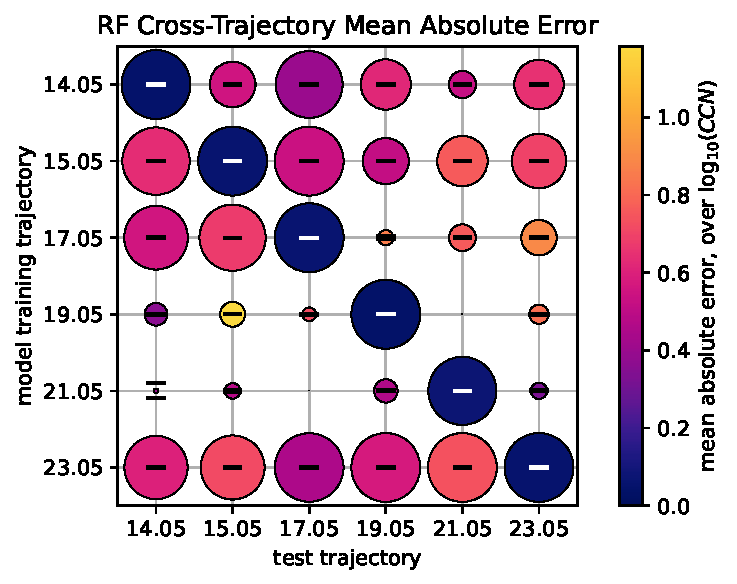
\includegraphics[width=0.425\textwidth]{evaluation/figures/results/trajectory-generalisation-rf-mae.pdf}
    \end{subfigure}
    \begin{subfigure}
        \centering
        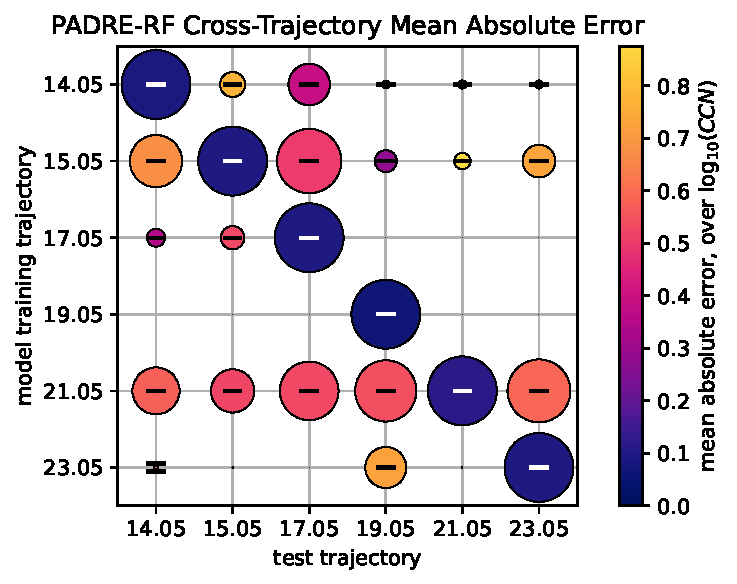
\includegraphics[width=0.425\textwidth]{evaluation/figures/results/trajectory-generalisation-padre-rf-mae.pdf}
    \end{subfigure}

    \begin{subfigure}
        \centering
        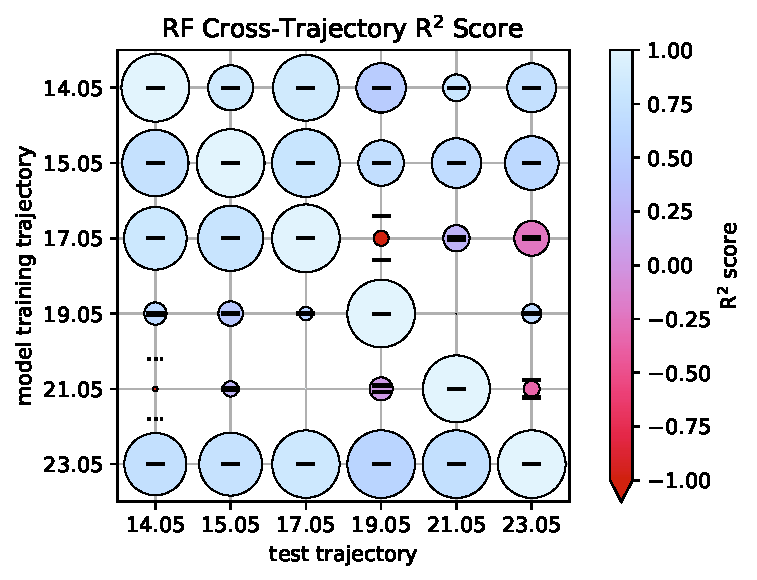
\includegraphics[width=0.425\textwidth]{evaluation/figures/results/trajectory-generalisation-rf-r2.pdf}
    \end{subfigure}
    \begin{subfigure}
        \centering
        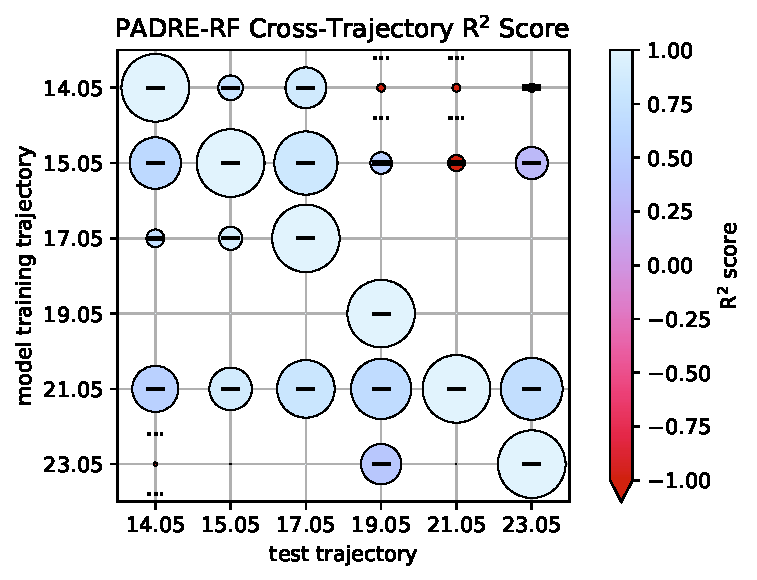
\includegraphics[width=0.425\textwidth]{evaluation/figures/results/trajectory-generalisation-padre-rf-r2.pdf}
    \end{subfigure}

    \caption[Evaluation of the SOSAA RSM across Six Trajectories]{Evaluation of the SOSAA RSM across the six trajectories from \Cref{txt:six-trajectories} using heatmap plots. The rows represent the trajectory a model was trained on, and the columns show which trajectory it is tested on. Note that the training and test data are always disjoint. There is one circle per cell whose area represents the RSM's confidence. In the first row, the circle's colour encodes the prediction MAE using the CET-L8 colour scheme \cite{color-cet-2015, color-cet-2023}, which ranges from dark blue for zero error over red to yellow for high error. A black line indicates the maximum MAE on its axis. In the second row, the CET-L19 colour scheme \cite{color-cet-2015, color-cet-2023} encodes the $R^2$ score, ranging from light blue for the optimal $R^2 = 1$ score over purple to red. Note that the colour mapping clips $R^2$ scores below $-1.0$ for better readability. Each cell also shows the result's uncertainty $\pm \sigma$ error bars whose height is scaled to match the colour bar's scaling. If the uncertainty would exceed the size of a single matrix cell, the error bars are dotted.}
    \label{fig:sosaa-rsm-trajectories}
\end{figure}

\section{Limitations with Predicting Perturbations} \label{txt:perturbation-generalisation}

As a final stress test, we evaluate the performance of the SOSAA RSM on perturbed inputs. This final analysis is meant to uncover the current limitations of our proof-of-concept implementation and thus showcase where future research should be directed. For this final experiment, we have classified most input variables as belonging to one of the following eight perturbation groups (see also \Cref{app:sosaa-variables}):
\begin{enumerate}
    \item \textbf{ant:} anthropogenic emissions, excluding $\text{CO}$, $\text{NO}_{x}$, $\text{NH}_3$, $\text{CH}_4$, and $\text{SO}_2$
    \item \textbf{bio:} biogenic emissions, excluding $\text{CO}$, $\text{CH}_4$, $\text{CH}_2\text{Br}_2$, $\text{CH}_3\text{I}$, $\text{CHBr}_3$, $\text{DMS}$, and terpene emissions
    \item \textbf{aer:} aerosol emissions with diameters between $3\text{nm}$ and $1000\text{nm}$
    \item \textbf{mtp:} biogenic monoterpene emissions, including $\alpha$-pinene, $\beta$-pinene, and others
    \item \textbf{sqt:} biogenic sesquiterpene emissions
    \item \textbf{$\text{SO}_2$:} anthropogenic $\text{SO}_2$ emissions
    \item \textbf{$\text{NO}_{x}$:} anthropogenic $\text{NO}_{x}$ emissions
    \item \textbf{$T$:} air temperature
\end{enumerate}
\noindent We assign each group a small increase, small decrease, large increase, and large decrease operation. For the emissions, these are the multiplicative factors $\times 1.01$, $\div 1.01$, $\times 1.5$, and $\div 1.5$, respectively. For the air temperature, we use $+1.04\text{K}$, $-1.04\text{K}$, $+2\text{K}$, and $-2\text{K}$. We have performed each of these 32 perturbation combinations for each of the six example trajectories from \Cref{txt:six-trajectories} using the SOSAA model. \Cref{app:sosaa-perturbation-outputs} showcases the change in CCN concentration for each of these 192 perturbation runs, which are also included in the SOSAA trajectories dataset (see \Cref{txt:sosaa-data-chapter}). While we only treat these perturbation results as numerical test data in this chapter, we hope that these perturbation run comparisons also prove useful to atmospheric scientists.

In this section, we analyse whether the RSMs are able to (a) predict the change in CCN concentration given the perturbation of the inputs, or (b) reject these perturbations as OOD. This task is very difficult and aims to stress-test the RSMs. For this, we ask the RSM to predict both the CCN concentration for the baseline and the perturbed inputs. We then use confidence and uncertainty propagation (see \Cref{txt:icarus-propagation}) to combine both outputs and predict the CCN difference, as usual in $\log_{10}(CCN)$ space (see \Cref{txt:model-criteria}), and its uncertainty and confidence. The results are shown in \Cref{fig:sosaa-rsm-perturbations-rf-small} and \Cref{fig:sosaa-rsm-perturbations-rf-large} for the random forest and \Cref{fig:sosaa-rsm-perturbations-padre-rf} for PADRE-RF. The small and large perturbations are split into separate figures. The plots use the same visual language as \Cref{fig:sosaa-rsm-trajectories} to communicate confidence levels, the $R^2$ score, and its uncertainty.

\newpar \Cref{fig:sosaa-rsm-perturbations-rf-small} shows that the RF-based SOSAA RSM fails even for small perturbations. While most difference predictions have very low $R^2$ scores, the 15.05., 21.05., and especially the 23.05. trajectories fare slightly better. However, none achieve visibly better scores than $R^2 = 0$ and instead perform significantly worse. Most critically, the OOD detector fails to detect that the RSM is unable to make good predictions for these perturbations. In \Cref{fig:sosaa-rsm-perturbations-rf-large}, we can see that some significantly larger perturbations are finally assigned lower confidence scores. Interestingly, most of the worst $R^2$ scores are achieved for anthropogenic emissions and air temperatures. In \Cref{txt:feature-importance}, we identified these variables as the most important features to both random forests and PADRE-RF. We thus hypothesise that both the predictor and OOD detector have concluded that changes in these variables are in-distribution since they had high variation and explanatory value in the training data.

\begin{figure}[H]
    \centering
    \begin{subfigure}
        \centering
        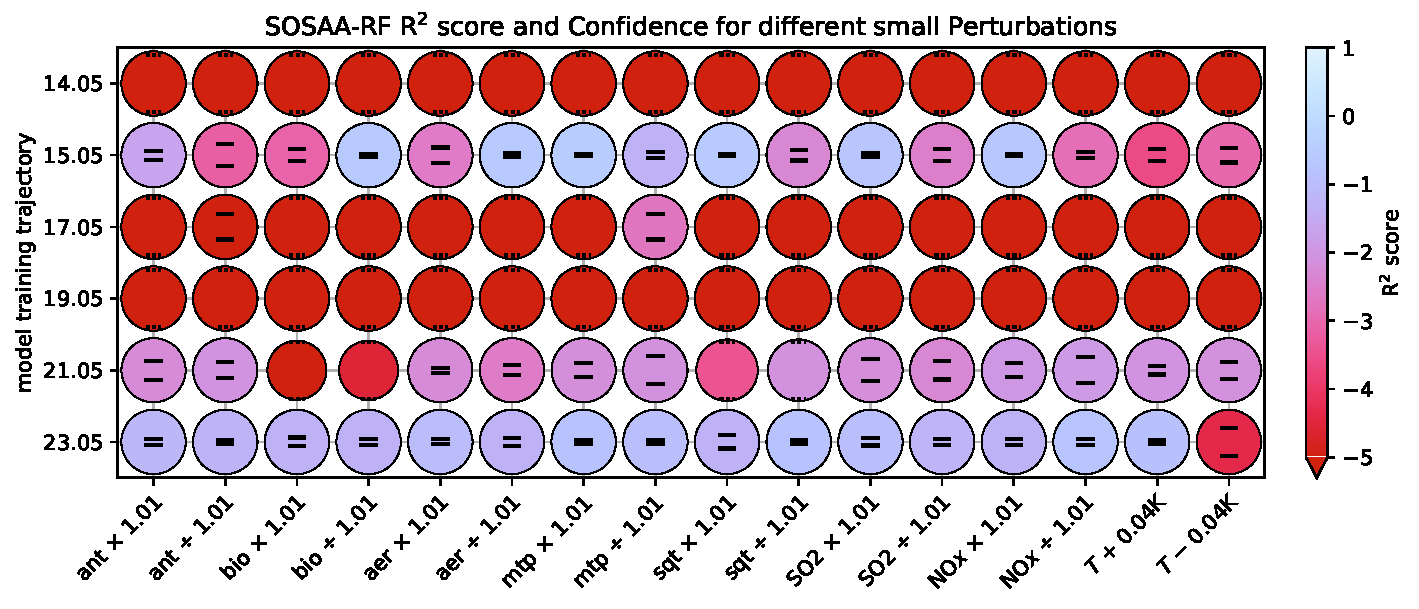
\includegraphics[width=0.95\textwidth]{evaluation/figures/results/perturbation-generalisation-rf-small.pdf}
    \end{subfigure}

    \vspace{-1em}
    \caption[Evaluation of the SOSAA-RF RSM on small Perturbations]{Evaluation of the SOSAA-RF RSM on small perturbations to the RSM's training trajectory. The rows represent the trajectory a model was trained on, and the columns show which perturbation is applied. The $R^2$ confidence, value, and uncertainty are encoded using circle area, colour, and error bar height, as in \Cref{fig:sosaa-rsm-trajectories}. Note that the colour mapping clips $R^2$ scores below $-5.0$ for better readability. The performance of the SOSAA-RF RSM on large perturbations is shown in \Cref{fig:sosaa-rsm-perturbations-rf-large}.}
    \label{fig:sosaa-rsm-perturbations-rf-small}
\end{figure}

\begin{figure}[H]
    \centering
    \begin{subfigure}
        \centering
        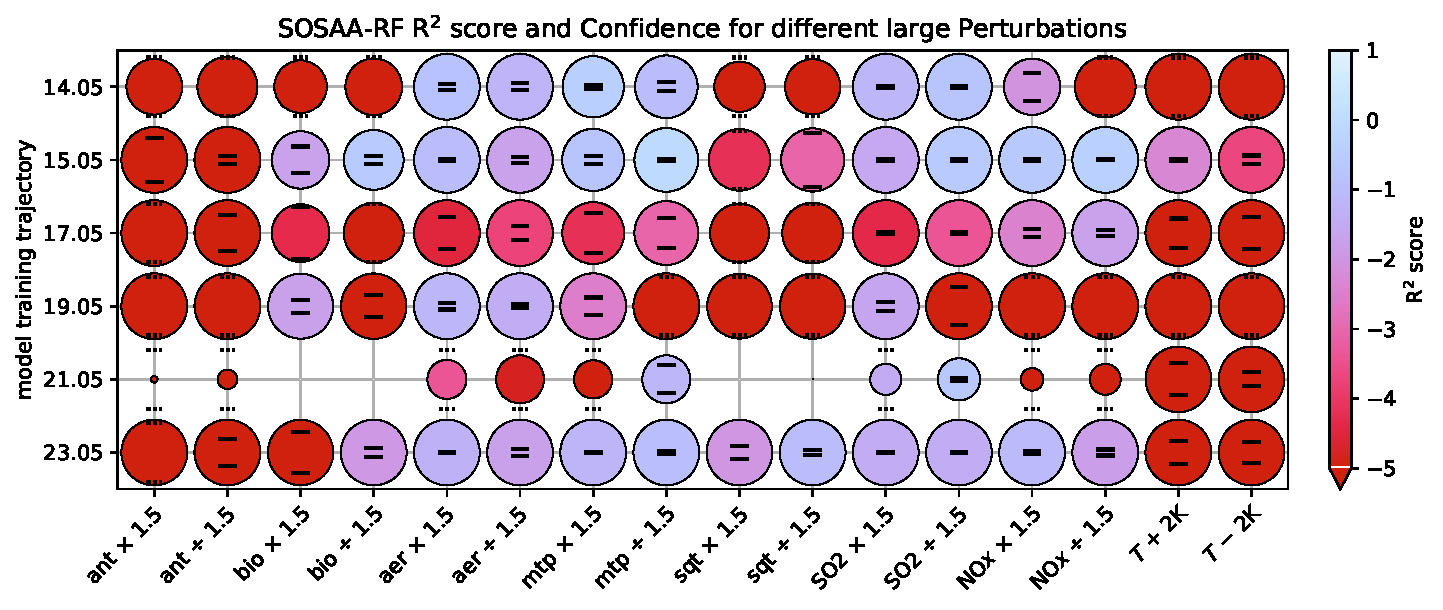
\includegraphics[width=0.95\textwidth]{evaluation/figures/results/perturbation-generalisation-rf-large.pdf}
    \end{subfigure}

    \vspace{-1em}
    \caption[Evaluation of the SOSAA-RF RSM on large Perturbations]{Evaluation of the SOSAA-RF RSM on large perturbations to the RSM's training trajectory. Please refer to \Cref{fig:sosaa-rsm-perturbations-rf-small}, the first half of this figure, for a description of the plot's encoding of $R^2$ confidence and uncertainty.}
    \label{fig:sosaa-rsm-perturbations-rf-large}
\end{figure}

\vspace{-1em}

\begin{figure}[H]
    \centering
    \begin{subfigure}
        \centering
        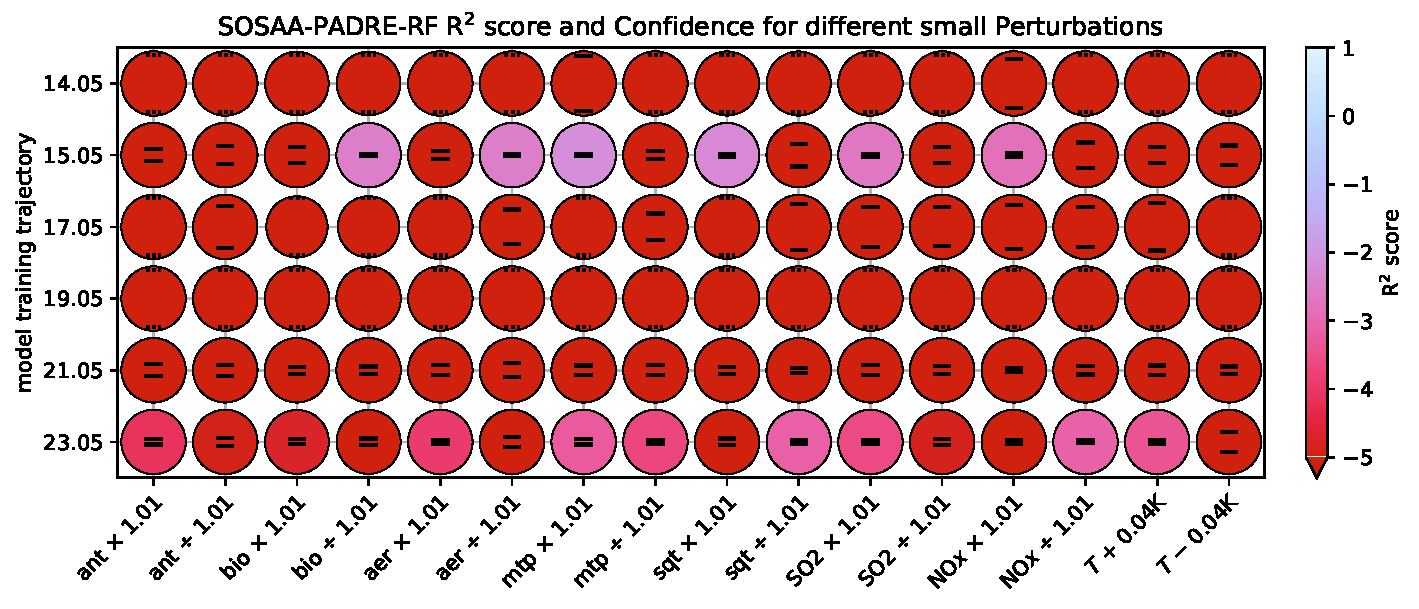
\includegraphics[width=0.95\textwidth]{evaluation/figures/results/perturbation-generalisation-padre-rf-small.pdf}
    \end{subfigure}

    \begin{subfigure}
        \centering
        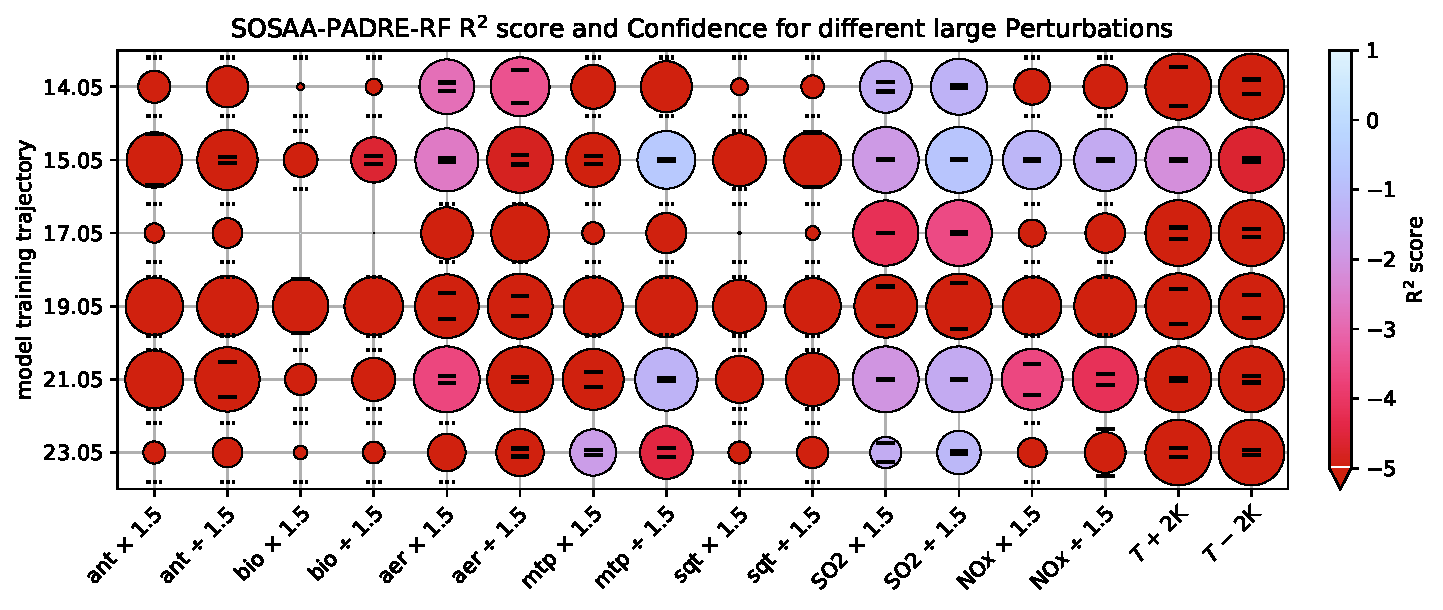
\includegraphics[width=0.95\textwidth]{evaluation/figures/results/perturbation-generalisation-padre-rf-large.pdf}
    \end{subfigure}

    \vspace{-1em}
    \caption[Evaluation of the SOSAA-PADRE-RF RSM on Perturbations]{Evaluation of the SOSAA-PADRE-RF RSM on perturbations to the RSM's training trajectory. The rows represent the trajectory a model was trained on, and the columns show which perturbation is applied. The $R^2$ confidence, value, and uncertainty are encoded using circle area, colour, and error bar height, as in \Cref{fig:sosaa-rsm-trajectories}. Note that the colour mapping clips $R^2$ scores below $-5.0$ for better readability. The upper chart covers the small perturbations, while the lower one contains the results for larger perturbations.}
    \label{fig:sosaa-rsm-perturbations-padre-rf}
\end{figure}

\noindent \Cref{fig:sosaa-rsm-perturbations-padre-rf} shows that PADRE-RF performs even worse at the predicting the change in CCN for different input perturbations. All small perturbations are assigned almost full confidence even though they also produce highly negative $R^2$ scores. One potential explanation for the worse scoring of PADRE-RF is the higher natural noise in its predictions. Since two such noisy predictions are combined, the predicted difference may be obscured. For larger perturbations, PADRE-RF produces slightly better $R^2$ scores, and its OOD detection on pairwise features is able to identify more inputs as OOD than the RF's OOD detector. However, even SOSAA-PADRE-RF is stumped by the temperature perturbations, which it classifies as ID.

\newpar How could the performance of the proof-of-concept SOSAA RSM be improved? We briefly test two small changes to the SOSAA RSM and report our preliminary results. First, the OOD detector is clearly overconfident on the perturbation inputs. While a future OOD detector could be specifically trained to detect OOD perturbations, we test a simpler approach and swap out the confidence scorer of the OOD detector. We had previously chosen to use confidence scores based on logistic regression since it produced the best calibration results in \Cref{txt:ood-logistic-scoring}. However, the fact that the scorer never assigned any intermediate confidence scores (see \Cref{fig:logistic-ood-scoring}) should have been a warning sign. A good confidence scorer for a \textit{prudent} RSM should not only correctly classify ID and OOD inputs but also be provably well-calibrated or at least underconfident on non-extreme scores. The upper row in \Cref{fig:sosaa-rsm-perturbations-improvements} shows that using the percentile-based confidence scorer with the otherwise unchanged SOSAA-PADRE-RF RSM detects many more inputs as OOD, at the cost of being generally quite underconfident.

\vspace{-1em}
\begin{figure}[H]
    \centering
    \begin{subfigure}
        \centering
        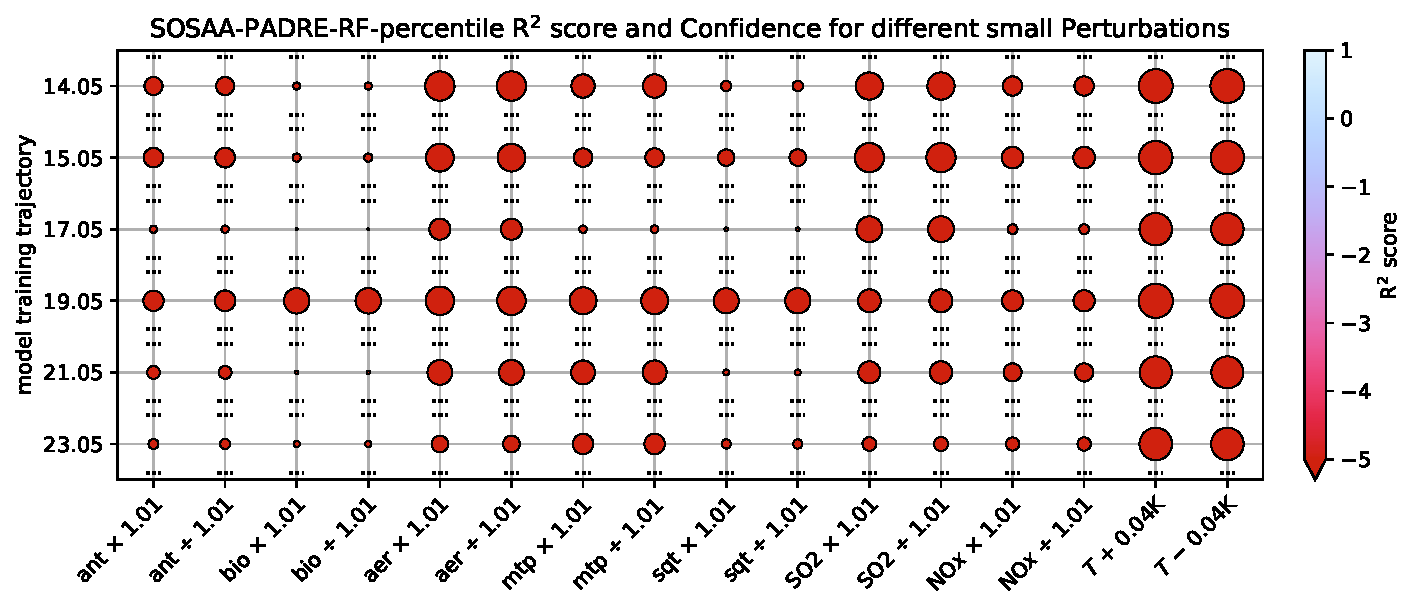
\includegraphics[width=0.95\textwidth]{evaluation/figures/results/perturbation-generalisation-percentile-padre-rf-small.pdf}
    \end{subfigure}

    \begin{subfigure}
        \centering
        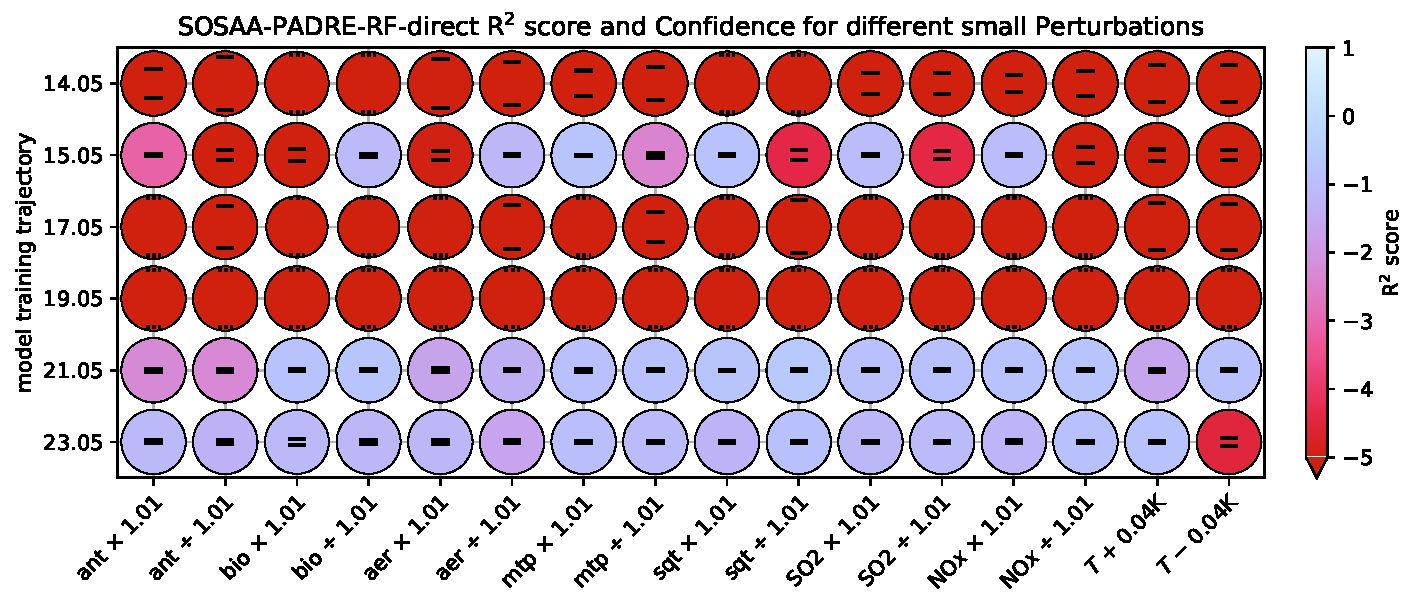
\includegraphics[width=0.95\textwidth]{evaluation/figures/results/perturbation-generalisation-padre-rf-direct-small.pdf}
    \end{subfigure}

    \vspace{-1em}
    \caption[Evaluation of Improvements to the SOSAA-PADRE-RF RSM]{Evaluation of potential improvements for the SOSAA-PADRE-RF RSM on perturbations to the RSM's training trajectory. The rows represent the trajectory a model was trained on, and the columns show which perturbation is applied. The $R^2$ confidence, value, and uncertainty are encoded using circle area, colour, and error bar height, as in \Cref{fig:sosaa-rsm-trajectories}. Note that the colour mapping clips $R^2$ scores below $-5.0$ for better readability. The upper chart shows SOSAA-PADRE-RF's performance on small perturbations when using the percentile-based confidence score (see \Cref{fig:percentile-ood-scoring}), while the lower chart showcases using PADRE-RF's direct perturbation predictions.}
    \label{fig:sosaa-rsm-perturbations-improvements}
\end{figure}

\newpar We have also briefly tested a second idea that aims to better utilise pairwise difference regression. Thus far, we have treated PADRE-RF no different than the RF predictor and simply asked it to produce one prediction on the baseline inputs and one on the perturbed inputs, before combining them using confidence and uncertainty propagation. However, combining two noisy predictions clearly does not produce well-correlated difference predictions. Therefore, we instead try to only apply PADRE-RF once, giving it the entire training trajectory and the exact perturbations as its non-random pairwise input $(X_{\text{train}}, X_{perturbed} - X_{\text{train}})$. Note that we can no longer average several predictions using this method. Remarkably, the bottom row of \Cref{fig:sosaa-rsm-perturbations-improvements} shows that this approach does indeed improve the quality of the perturbation-caused CCN difference predictions drastically, putting SOSAA-PADRE-RF on par or even above the SOSAA-RF RSM.

\newpar While we have also tried combining this approach with the percentile-based confidence scores, this combination did not result in any further improvements. Nevertheless, we hope these two preliminary ideas prove useful for future investigation into a SOSAA RSM that can successfully predict the effects of perturbations.

\newpar Finally, it is worth returning to our hypothesis in \Cref{txt:feature-importance}. Since PADRE-RF assigns higher feature importance to biogenic, monoterpene, and sesquiterpene emissions than the RF, we hypothesised that PADRE-RF might perform better at predicting perturbations for these features. Unfortunately, neither method produces different-quality predictions for these perturbations in comparison to the other groups. However, PADRE-RF's OOD detector does classify all biogenic perturbations to be more OOD than SOSAA-RF's one. Thus, we can only support the hypothesis for our OOD detection but not for our prediction model implementation.

\section{Conclusions on the SOSAA RSM} \label{txt:sosaa-rsm-conclusions}

In this chapter, we have constructed a proof-of-concept SOSAA RSM built on the Icarus architecture. Based on our investigation of out-of-distribution detectors, prediction models, and uncertainty quantifiers in \Cref{txt:ood-detection-chapter}, \Cref{txt:prediction-chapter}, and \Cref{txt:uncertainty-chapter}, respectively, we have combined some of the best-performing yet also computationally efficient components to assemble a random-forest (RF) and a PADRE-RF based RSM. We evaluated how much these RSMs rely on spatiotemporal memory of their training trajectory and how well they perform on time-adjacent and unrelated other trajectories. Finally, we have tested if they can also be applied to predict the effect of perturbations. In particular, we have seen that while the RF-based RSM's performance degenerates quickly on test data outside the training trajectory, PADRE-RF is noisier in general but also performs more robustly with higher clumping, on adjacent and unrelated trajectories. Furthermore, using an OOD detector whose inputs explicitly include the distance to training inputs, as is the case for the pairwise inputs, allows the detector to detect OOD inputs more precisely.

\newpar However, our final stress test of the RSMs on input perturbations has shown that our proof-of-concept implementations are still severely limited. It is tempting to wonder if perhaps SOSAA's perturbation results are wrong and the RSM's predictions are correct. However, throughout this thesis, we have treated the SOSAA model's results as the ground truth. Even though predicting small perturbations is a very difficult task, a prudent RSM should either be able to replicate the model's behaviour or decrease its confidence for such inputs that fall outside the conceptual training data manifold. While using the Icarus RSM architecture allows the RSMs to catch some cases where they should not make a prediction, the logistic regression-based OOD detector, which we chose due to its excellent performance in \Cref{txt:ood-logistic-scoring}, is severely overconfident on the perturbation inputs. If an RSM is to be primarily applied to such perturbations, the OOD detector should be specifically trained on synthetic OOD perturbations. The ID vs OOD weighting method from \Cref{txt:id-ood-weighting} may then be used during training to avoid overlap between ID and OOD samples. Furthermore, a \textit{prudent} RSM should prefer using an underconfident scoring function such as the percentile score (see \Cref{txt:percentile-confidence}). We have briefly investigated two small adjustments to the SOSAA RSM and shown that percentile-based confidence scores (see \Cref{txt:percentile-confidence}) and direct perturbation predictions can indeed both improve the performance of the SOSAA-PADRE-RF RSM.

Our stress test has also clearly shown that the chosen simple prediction models, which are only trained on the baseline trajectory, are generally insufficient to make perturbation predictions. Future work could investigate whether combining the baseline trajectory with the SOSAA outputs from a single targeted general perturbation run may be enough to improve the predictor, as suggested by \textcite{deep-rsm-2020}.

\newpar Next up, \Cref{txt:sosaa-gui-chapter} introduces the SOSAA GUI, which we have developed during this project to make future development on and research with SOSAA easier. In addition to providing an intuitive interface for configuring the SOSAA model, it also has support for training and using the SOSAA RSM and can thus serve as a testbed for future improvements to the RSM and its use.
